\chapter{Modelo de Seguridad de Android}
Android \cite{aos} es un sistema operativo \textit{open-source} \cite{aosp} diseñado para dispositivos móviles y
desarrollado por Google junto con la Open Handset Alliance \cite{oha}. Su arquitectura sigue el estilo arquitect\'onico conocido como Sistemas Estratificados: los distintos componentes se agrupan en capas seg\'un su nivel de abstracci\'on, conformando una jerarqu\'ia. Las capas inferiores contienen componentes ligados al \textit{hardware}, mientras que las capas superiores agrupan componentes ligados con tareas de m\'as alto nivel.\\
Una de las características principales de Android es que cualquier aplicación, ya sea principal o
creada por algún desarrollador, puede, al instalarse con las autorizaciones adecuadas, utilizar tanto
los recursos/servicios del dispositivo móvil como los ofrecidos por el resto de las aplicaciones
instaladas.\\
A lo largo de este cap\'itulo se har\'a una descripci\'on de los principales aspectos del modelo de seguridad de Android, basandose en la versi\'on 6.0 llamada Marshmallow, lanzada en 2015.
\section{Características agregadas en Android Marshmallow}
\subsection{Entorno aislado para cada aplicaci\'on}\label{ch01-sandbox}
Fue una de las primeras tecnologías de seguridad aplicadas en Android, y tiene mucha importancia en el modelo de seguridad. Consiste en que cada aplicaci\'on se ejecuta en un entorno aislado (\textit{sandbox}), forzando a que solo pueda tener acceso irrestricto a sus propios recursos. Por lo tanto, las aplicaciones no pueden interactuar entre ellas y tienen acceso limitado al sistema operativo. Adem\'as, se les asigna una única id de usuario (UID) y se ejecutan en ese usuario como un proceso independiente, como se observa en la Figura \ref{fig:ch01:sandbox}.\\
Como el entorno aislado está en el \textit{kernel}, este modelo de seguridad se extiende al código nativo y a las aplicaciones del sistema operativo, tales como las bibliotecas del sistema operativo y los \textit{frameworks} de las aplicaciones. Esto genera un aislamiento a nivel del \textit{kernel}, ya que todas las políticas que se aplican a usuarios o grupos de usuarios, se trasfieren a las aplicaciones por tener su UID.
\begin{figure}[!hb]
	\begin{center}
		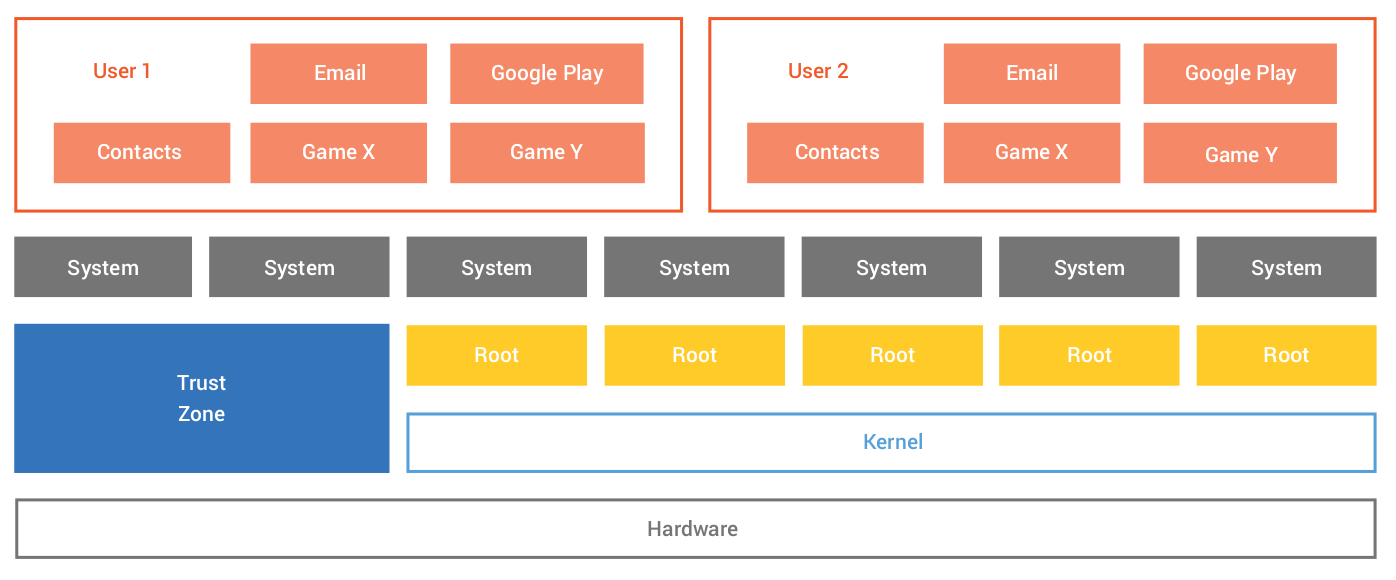
\includegraphics[width=0.75\linewidth]{chapter1/android_security_model}
	    \caption{Ailamiento de las aplicaciones seg\'un su UID \cite{asreview2015}.}
	    \label{fig:ch01:sandbox}
    \end{center}
\end{figure}
\subsection{Pol\'iticas de acceso mejoradas}
\emph{SELinux}(por sus siglas en ingl\'es \textit{Security-Enhanced Linux}) es un sistema de políticas de acceso obligatorio para Linux. Es decir, siempre se consulta con una autoridad central para permitir cualquier acceso a un recurso; esto abarca a todos los procesos, inclusive aquellos que corren con privilegios de \textit{root}.\\
Decimos que un dominio es una etiqueta que identifica un conjunto de procesos en una política de seguridad. Los procesos que comparten una misma etiqueta de dominio son tratados de la misma forma. \\
\emph{SELinux} opera bajo \textit{the ethos of default denial}, es decir, todo lo que no está explícitamente permitido es denegado. Puede trabajar en dos modos:
\begin{itemize}
    \item \underline{Riguroso:} aplica estrictamente las políticas de seguridad.
    \item \underline{Permisivo:} no se aplican las políticas pero se guardan en un log.
\end{itemize} 
Se permite aplicar el modo permisivo en un determinado dominio y el resto del sistema permanece en modo riguroso. Por lo tanto, se puede lograr una aplicación incremental de \emph{SELinux} a una porción cada vez mayor del sistema y desarrollar de políticas para nuevos servicios (manteniendo el resto del sistema en vigencia).
\subsection{Arranque seguro}
\begin{figure}[!hb]
	\begin{center}
		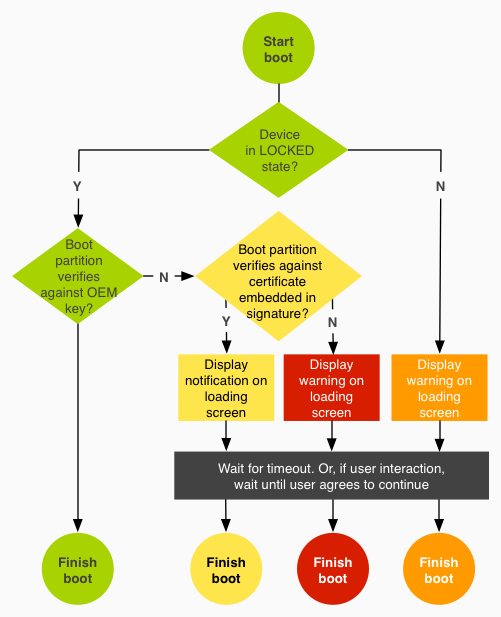
\includegraphics[width=0.5\linewidth]{chapter1/verified_boot}
		\caption{Diagrama de flujo del Verified Boot \cite{aossec}}
		\label{fig:ch01:verifyBoot}
	\end{center}
\end{figure}
Esta funcionalidad garantiza un arranque seguro del dispositivo, comenzando desde un lugar confiable del \textit{hardware} hasta que se monta la partición. Durante el booteo, el sistema operativo chequea que la versión de Android no se haya alterado respecto a la de fábrica, informando mediante alertas en caso contrario y ofreciendo opciones para resolverlo.\\
Dependiendo de la implementación de la funcionalidad, el sistema operativo puede ofrecer una acción al usuario o evitar el arranque hasta que se haya solucionado el problema. En la figura \ref{fig:ch01:verifyBoot} se observa el diagrama de flujo del Arranque seguro, el cual termina en cuatro estados posibles:
\begin{itemize}
	\item Verde: indica que se pudo verificar correctamente el arranque del sistema.
	\item Amarillo: indica que se pudo validar el certificado embebido, correspondiente a la partición de booteo. Requiere la huella dactilar para continuar el inicio.
	\item Naranja: indica que el dispositivo pudo ser modificado, ya que no se pudo verificar la partición de booteo. Requiere acción del usuario para continuar.
	\item Rojo: indica que falló la verificación. Es decir, no pudo validar ninguna partición.
\end{itemize}
\subsection{Cifrado de la partici\'on de datos}
El cifrado es el proceso de codificación de todos los datos de usuario en un dispositivo Android utilizando claves de cifrado simétricas. Una vez que se encripta un dispositivo, todos los datos creados por el usuario se cifran automáticamente antes de enviarlos al disco y todas las lecturas descifran automáticamente los datos antes de devolverlos al proceso de llamada. Al arrancar, el usuario debe proporcionar sus credenciales antes de acceder a cualquier parte del disco.\\
La primera vez que apareció fue en la versión 3.0, pero recién a partir de la versión 5.0 fue fuertemente recomendado a los fabricantes de dispositivos que habiliten esta característica para todos sus dispositivos. La novedad incorporada en Android Marshmallow es que se puede encriptar la tarjeta SD, permitiendo que sea ilegible si es removida del dispositivo. Al habilitar esta opci\'on, por defecto se encriptan los datos privados de las aplicaciones, el contenido de la tarjeta SD y los datos personales.
\subsection{Autenticaci\'on del usuario}
Android provee diversas formas para que un usuario se autentique, permitiendo así desbloquear la pantalla. Desde los comienzos, la autenticaci\'on se realizaba mediante el PIN, contraseña y patrones. A partir de la versión 5.0, se introduce el concepto llamado \textit{TrustAgents}, el cuál permite mecanismos de desbloqueo más flexibles, tales como:
\begin{itemize}
	\item Reconocimiento facial.
	\item Un determinado lugar, configurado a través de Google Maps.
	\item Reconocimiento de vos.
	\item Ciertos dispositivos, tales como el auto (a través de Bluetooth).
\end{itemize}
La novedad en la versión 6.0 es que soporta el lector de huellas digitales.\\
\begin{figure}[!ht]
	\begin{center}
		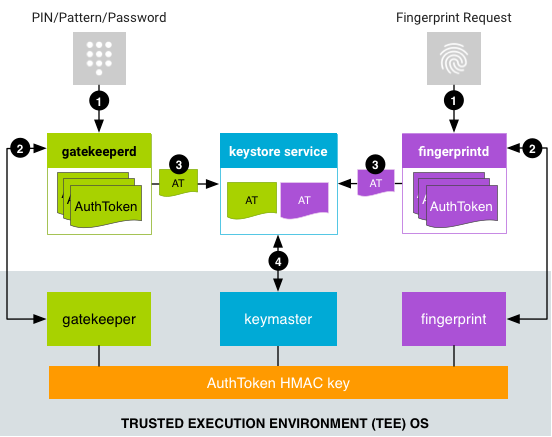
\includegraphics[width=0.5\linewidth]{chapter1/authentication-flow}
		\caption{Diagrama de flujo del proceso de autenticaci\'on \cite{aossec}}
		\label{fig:ch01:authentication-flow}
	\end{center}
\end{figure}
Como se observa en la Figura \ref{fig:ch01:authentication-flow}, la verificación del desbloqueo de la pantalla ocurre en el TEE \footnote{El \textit{Trust Execution Enviroment}(TEE) es una zona segura del procesador principal en la cual se provee una ejecución segura e íntegra, tanto de código fuente como de datos. El TEE aísla por \textit{hardware} el acceso a cierta memoria y provee mecanismos de I/O para dicha memoria \cite{tee2011}.}.
Dependiendo del método utilizado para autenticarse, el sistema operativo provee \textit{Gatekeeper}\footnote{El componente \textit{Gatekeeper} realiza la autenticación del patrón/contraseña del dispositivo en un entorno de ejecución de confianza (TEE). \textit{Gatekeeper} se inscribe y verifica las contraseñas a través de un HMAC con una clave secreta respaldada por \textit{hardware}.}, \textit{Fingerprint}\footnote{Es el componente encargado de verificar que la huella detectada por el sensor es v\'alida.}, \textit{Keystore}\footnote{Es un componente para almacenar las claves criptográficas, el cual dificulta su extracción, ya que asegura que una clave nunca entra en una aplicación y una clave nunca sale de una zona segura.\cite{dakss}} y otros componentes para soportar el uso de \textit{tokens} de autenticación respaldados por \textit{hardware} (\textit{AuthTokens}).\\
Como consecuencia del esta forma de autenticarse, se destacan las siguientes ventajas:
\begin{itemize}
    \item Al permitir el desbloqueo con datos biométricos, se acelera y se simplifica el proceso de autenticaci\'on. Los usuarios eligen este sistema de desbloqueo en un 91\% \cite{asreview2015}.
    \item Al realizarse la autenticaci\'on en un TEE, se mejora la protección contra ataques de fuerza bruta, ya que se incrementa exponencialmente el tiempo de espera para el desbloqueo \cite{asreview2015}.
\end{itemize}
Estas mejoras permiten que los desarrolladores de aplicaciones tengan más opciones de seguridad para sus datos y sus comunicaciones.
\section{Seguridad en las aplicaciones}
\subsection{Permisos} \label{ch01-permisos}
Ciertos recursos que provee Android son sensibles, ya que acceden a datos personales o periféricos importantes. Dichos recursos sólo pueden ser accedidos mediante una \textit{security-sensitive API}(SS-API por sus siglas en inglés) con un doble objetivo: tenerlos aislados y permitir cierta granularidad de seguridad sobre ellos \cite{HYGZD2014}.\\
\begin{figure}[hbtp]
	\begin{center}
		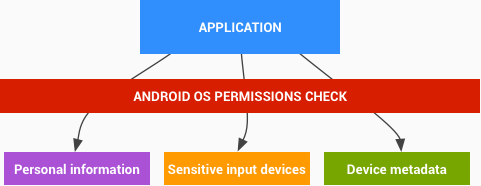
\includegraphics[width=0.75\linewidth]{chapter1/permissions_check}
		\caption{Los recursos solamente pueden ser accedidos a través de los permisos}
		\label{fig:ch01:permissions-check}
	\end{center}
\end{figure}
El mecanismo de seguridad para el acceso a estas SS-API de recursos se llama Permisos y se clasifican de acuerdo con el riesgo implícito al otorgarlos en las siguientes cuatro categorías:
\begin{itemize}
    \item \emph{Normal:} Son aquellos permisos de bajo riesgo ya que corresponden a características aisladas y son considerados de bajo riesgo para las demás aplicaciones, para el sistema y para el usuario. Son concedidos automáticamente por el sistema, sin solicitar aprobación explícita del usuario \cite{Rom14}.
    \item \emph{Dangerous:} Son aquellos permisos de alto riesgo ya que resguardan los accesos a información sensible para el usuario u otorgan control sobre funcionalidades principales del sistema. Para ser concedidos se requiere aprobación explícita del usuario \cite{Rom14}. 
    \item \emph{Signature:} Son aquellos permisos que son aprobados solamente si la aplicación que los requiere tiene el mismo certificado que la aplicación que los creó. Cuando el sistema valida el certificado, se otorga el permiso sin requerir aprobación explícita del usuario. Se crearon para permitir que un desarrollador pueda compartir información entre sus distintas aplicaciones sin necesidad de la aprobación del usuario \cite{Rom14}.
    \item \emph{Signature/System:} Son aquellos permisos que controlan el acceso a servicios críticos del sistema. En general, las únicas aplicaciones que los utilizan son las que vienen pre-instaladas en el dispostivo, ya que se utilizan para ciertas situaciones especiales en las que varios proveedores tienen aplicaciones integradas en una imagen del sistema que necesitan compartir funciones específicas explícitamente porque se están creando juntas \cite{Rom14}.
\end{itemize}
En el presente informe, nos centraremos en los permisos \emph{Normal} y \emph{Dangerous}; cómo se otorgan y cómo se deniegan.
\subsection{Manifiesto}
El archivo de manifiesto proporciona información esencial sobre tu aplicación al sistema Android, información que el sistema debe tener para poder ejecutar el código de la app. Es por ello, que todas las aplicaciones deben tener un archivo \texttt{AndroidManifest.xml} (con ese nombre exacto) en el directorio raíz. En este archivo se declaran todos los componentes que forman parte de la aplicación en cuestión, los permisos que son requeridos (ver sección \ref{ch01-permisos}) y los permisos exportados por la aplicación, entre otras cosas.
\begin{figure}[hbtp]
    \centering
    \lstinputlisting[language=XML, basicstyle=\tiny, breaklines=true, frame=single]{AndroidManifest.xml}
    \caption{Manifiesto de la aplicación que contiene los tests.}
    \label{fig:ch01:manifest}
\end{figure}